
\begin{figure}
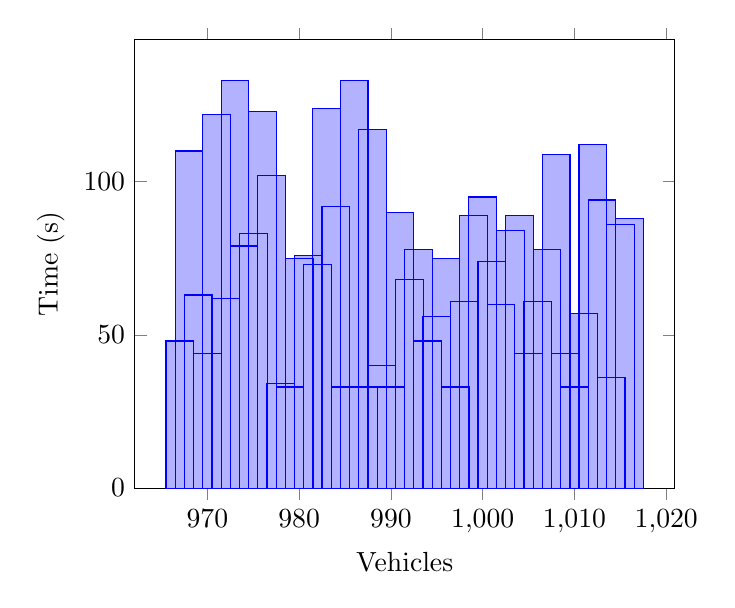
\begin{tikzpicture}
\begin{axis}[
legend style={anchor=west},
xlabel=Vehicles,
ylabel=Time (s),
ymin=0,
ybar,
]
\addplot coordinates {
(1014, 36)
(1015, 86)
(1016, 88)
(1010, 33)
(1012, 112)
(1013, 94)
(1004, 89)
(1002, 60)
(1000, 95)
(1006, 61)
(1009, 44)
(1008, 109)
(1007, 78)
(1005, 44)
(1001, 74)
(977, 102)
(976, 123)
(975, 83)
(974, 79)
(973, 133)
(972, 62)
(971, 122)
(970, 44)
(979, 33)
(978, 34)
(995, 56)
(994, 48)
(997, 33)
(996, 75)
(991, 90)
(990, 33)
(993, 78)
(992, 68)
(999, 89)
(998, 61)
(1011, 57)
(1003, 84)
(967, 48)
(968, 110)
(969, 63)
(987, 33)
(988, 117)
(989, 40)
(982, 73)
(983, 124)
(980, 75)
(981, 76)
(986, 133)
(984, 92)
(985, 33)
};

\end{axis}
\end{tikzpicture}
\label{tik:time:100:90}
\caption{100 percent diving with GSC on route $90$}
\end{figure}
